\subsubsection{Arquitectura del Sistema de Visión por Computadora}

El sistema de visión por computadora se estructura en tres módulos especializados que operan de manera coordinada durante los procesos de exploración y cosecha:

\textbf{Detector de Tubos de Cultivo:} Identifica tubos de PVC mediante análisis de bordes y saturación durante el escaneo vertical del workspace. Utiliza el algoritmo de Canny combinado con filtrado en el canal de saturación (HSV) para detectar los bordes superior e inferior de cada tubo. Registra las posiciones verticales Y de todos los tubos detectados, generando un archivo configuracion\_tubos.json que permite al sistema ubicar cada fila de cultivo.

\textbf{Detector de Cintas de Referencia:} Localiza cintas negras adhesivas de 18mm de ancho mediante umbralización inversa del canal V (HSV). Opera en tres contextos: corrección de posición horizontal (centroide de cinta vertical), corrección de posición vertical (arista base de cinta), y escaneo horizontal para registrar posiciones X de plantas en matriz\_cintas.json.

\textbf{Clasificador Morfológico de Cultivos:} Determina el estado de madurez mediante análisis del área de vegetación verde segmentada. Aplica umbralización en el espacio HSV para extraer píxeles verdes, refinamiento morfológico (cierre y apertura), detección de contornos, y clasificación por umbral de área estadísticamente determinado. Discrimina entre lechugas maduras (área mayor al umbral), plantas inmaduras, y posiciones vacías.

\begin{figure}[h]
\centering
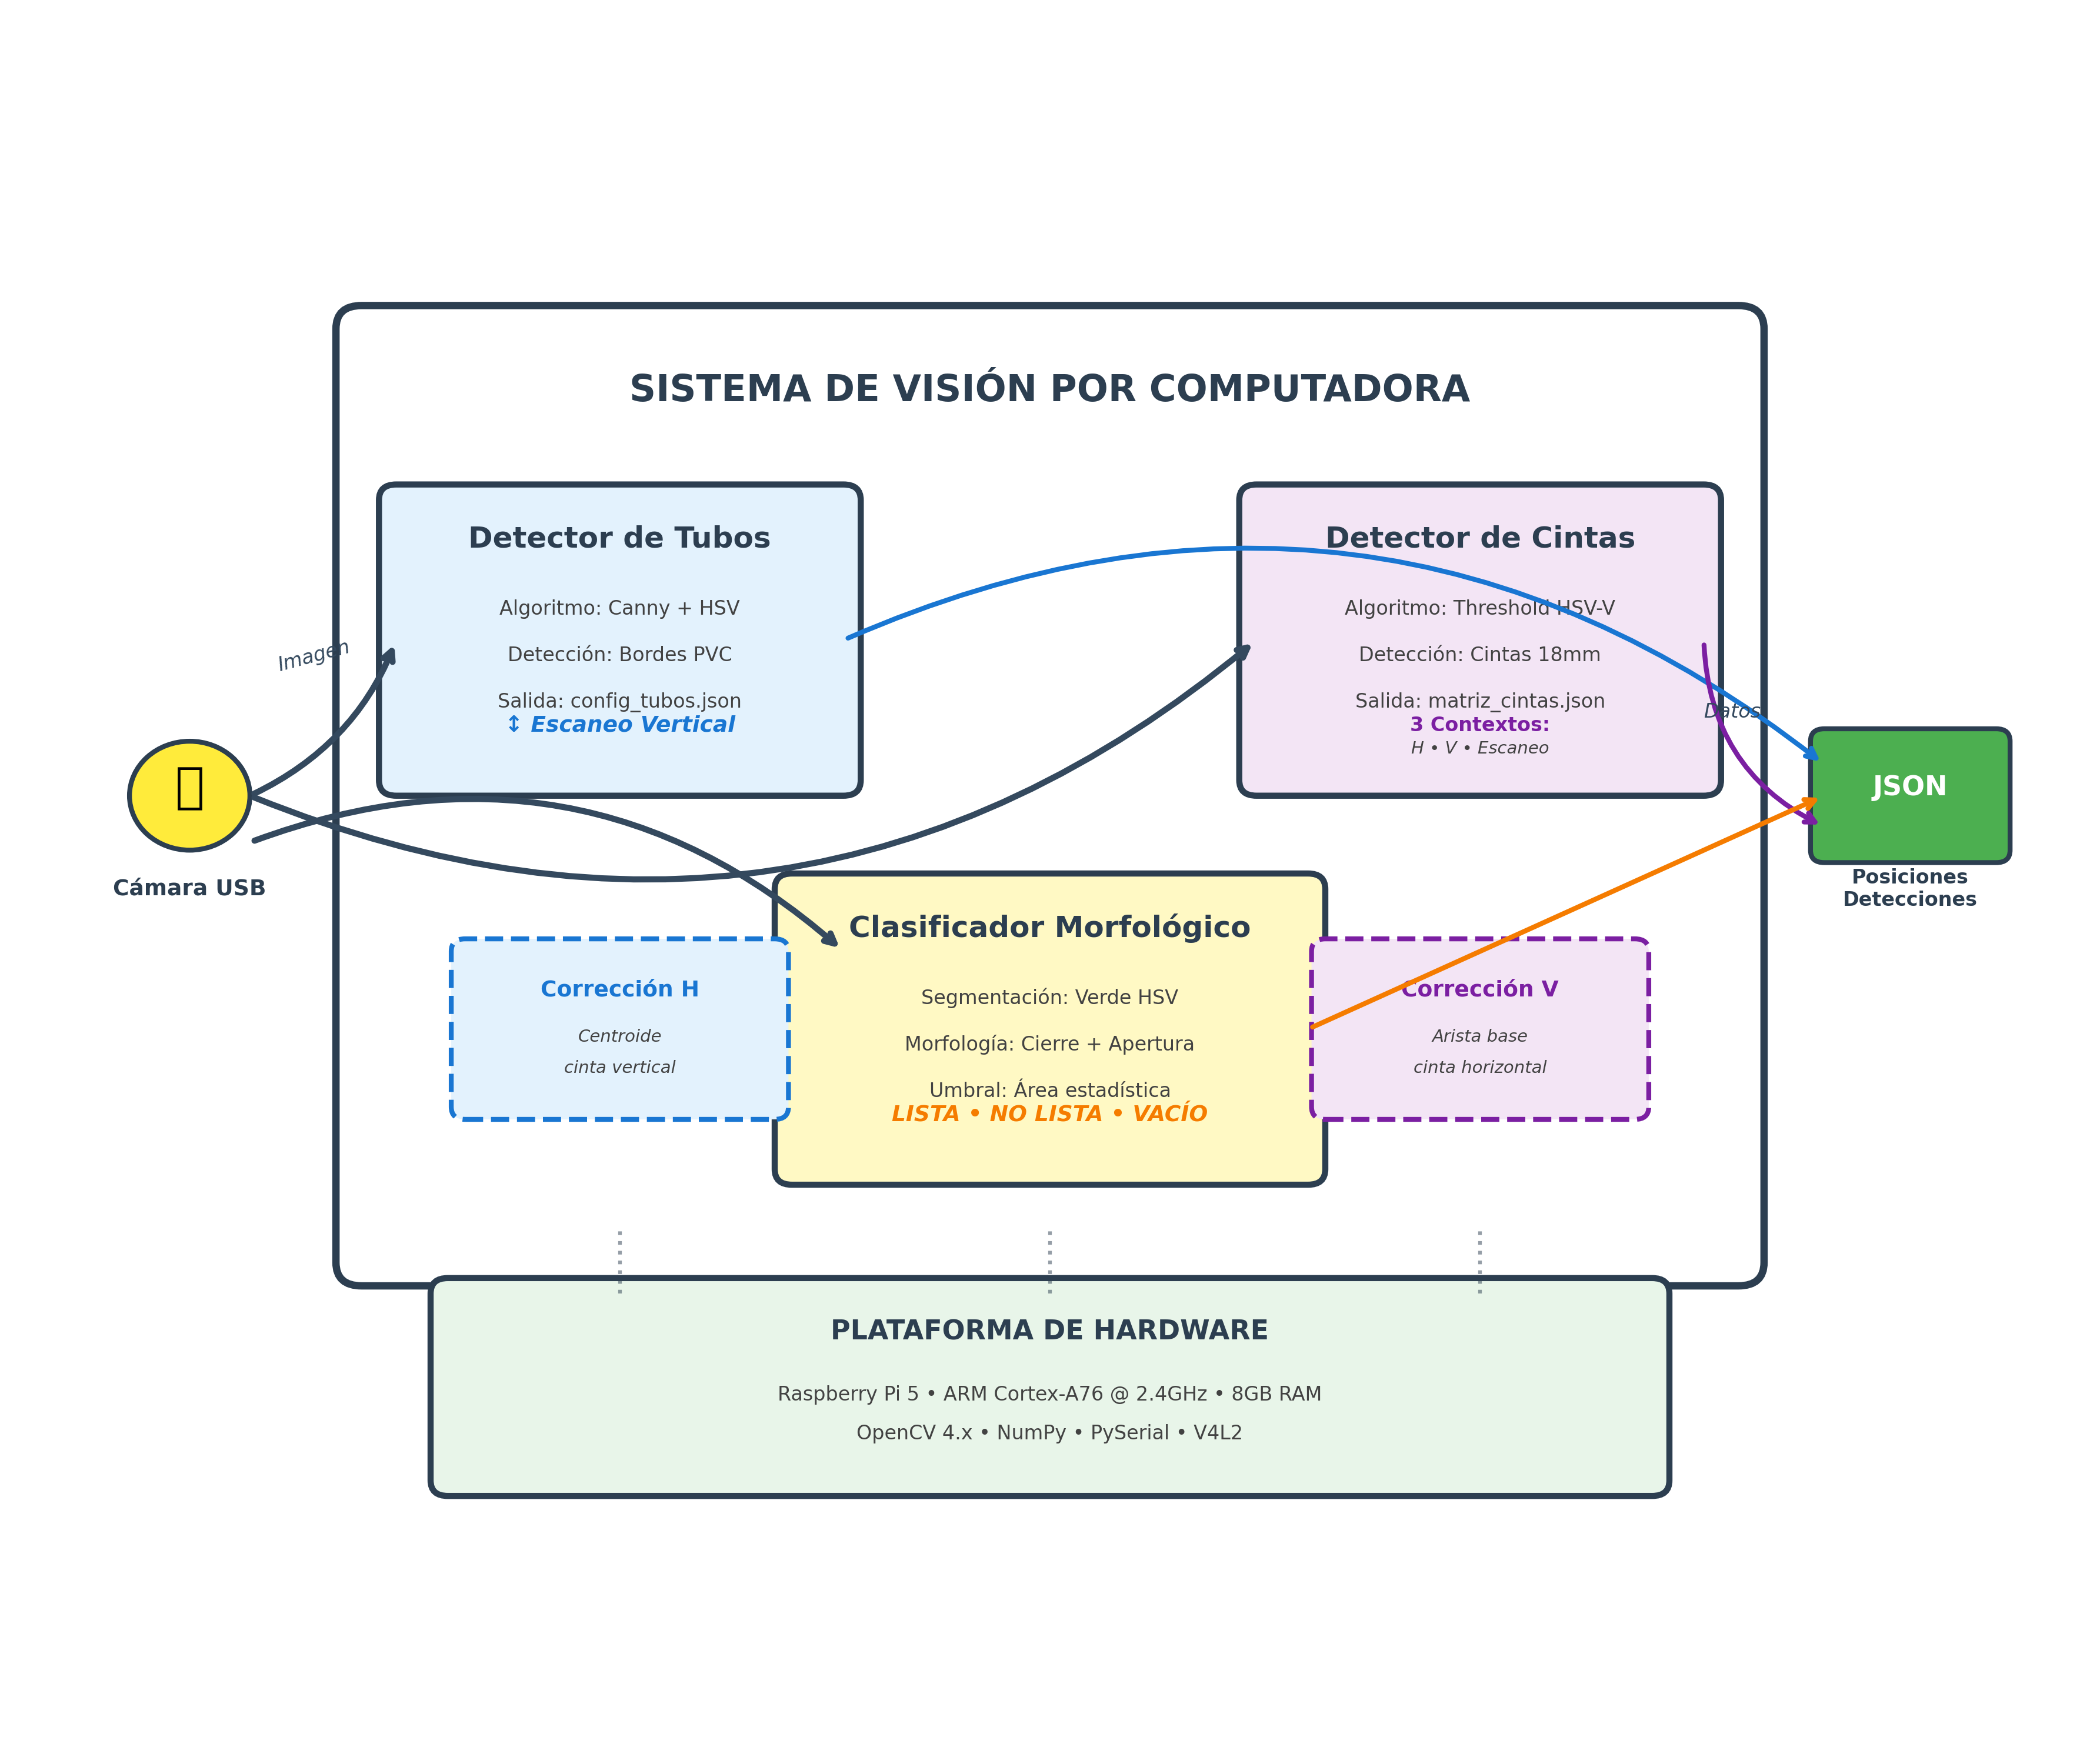
\includegraphics[width=0.85\textwidth]{imagenes/arquitectura_modular_vision.png}
\caption{\textit{Arquitectura modular del sistema de visión por computadora}}
\label{fig:arquitectura_modular}
\end{figure}

El sistema se implementa sobre Raspberry Pi 5 con procesador ARM Cortex-A76 quad-core a 2.4GHz y 8 GB de memoria RAM LPDDR4X. Las bibliotecas empleadas incluyen OpenCV 4.x para algoritmos de procesamiento de imágenes (Canny, morfología, detección de contornos), NumPy para operaciones matriciales eficientes sobre arreglos de píxeles, y PySerial para comunicación UART con el nivel regulatorio. El sistema operativo Raspberry Pi OS proporciona soporte nativo para el controlador V4L2 de la cámara USB.